\documentclass[template.tex]{subfiles}

\usepackage{comment} 

\begin{document}

\ref{Figure:phydraschematics}


 %% \ SECTION 3
\section{Use cases} \label{Section:UseCases}

\begin{comment}

Andrew Comments:

Structure: just go through it, Use Case I, Use Case II, Use Case II. No Methods & Results Section

go through it from front to back, explain what an NPZD model is.
"We recreate the NPZD model formulation by Anderson, in the model there is one .." describe equations in words. Then say See Anderson et al. or appendix X for full equations


%  quickly explain overview, explain methods for all of them shortly, with schematics, and put full system of equations & parameter tables in the Appendix!

TODO b4 handing in 2 esteban:
- fix the legend missing in NPZDslab Figure

\end{comment}

% PARAGRAPH STARTS HERE:


% in final version, present: - jupyter notebook for each example, add links in text

% idea I had is that I actually present the models phydra style, as a collection of different processes
% a) physical env (this handles forcing)
% b) components
% c) fluxes
% d) xs.Model, xs.create_setup, xsimlab.run()

Phydra is an object-oriented Python package for developing marine ecosystem models in a flexible modular structure. As an extension of the xarray-simlab package, phydra is embedded in the python scientific ecosystem and provides a collection of tool-sets for rapid prototyping, analysis \& visualisation of models. 

To showcase this utility, we present three model use cases of varying ecosystem complexity. In this section, we present simplified descriptions of model structure and mechanisms, following the model development workflow presented in Section \ref{Section:phydrapackage}.
Per use case, we first describe the generic physical environment employed. The environment collects the model components and computes common forcing fluxes. After describing the model components and what they represent, we move on to describe the fluxes that define the interactions between components. Finally, setup \& parameters for the model runtime are presented and simulation results are shown.

For a complete structure-independent mathematical description of the presented models please see Appendix 1. Additionally model and analysis code for all use cases is publicly available as documented interactive jupyter notebooks in the phydra repository (\url{https://github.com/ben1post/phydra/tree/master/examples}). \\

\subsection{Use case 1: a NPZD slab model}
Our first use case presents a classical NPZD model embedded in a "slab" physical setting. The simplified two-layer structure provides a zero-dimensional and mechanistically simple description of physical processes affecting euphotic ecosystems in the open ocean. The classical structure lends itself well as an efficient physical test-bed for more complicated ecosystem descriptions and is often used as a teaching example.
\\
The presented model is a slightly modified version of the elegant EMPOWER model, as presented by \citet{Anderson2015c}. 
The modifications we introduced were aimed at simplifying the description of the physical environment and the parameterisation of phytoplankton growth. 
Specifically our model formulation uses empirical forcing for irradiance (PAR) and nutrient concentration of the deep layer (\unit{N^\emptyset}). We chose to use Steele's formulation to represent light-limitation of phytoplankton growth in the mixed layer independent of chlorophyll biomass, as adapted from \cite{Acevedo-Trejos2016}.

See Figure \ref{Figure:phydraschematics_1} (a) for a schematic of the model structure and please refer to Appendix 1.1 for the full system of equations.


\subsubsection{Physical environment}
% a) physical env (this handles forcing)
The physical environment of a phydra model (hereafter referred to simply as environment) describes an xarray-simlab process that provides an interface for model forcings and methods for generalised forcing fluxes (e.g. mixing) in the Phydra package (see Section \ref{Section:PhysicalEnvironment} for details on phydra environments).
The environment of use cases 1 is a 'slab' description of an open ocean water column that is compatible with four types of external forcings: an external nutrient supply from below the mixed layer, (\unit{N^\emptyset}), depth of the mixed layer (MLD), photosynthetically active incident radiation (PAR) and average temperature above the mixed layer depth (\unit{T_{MLD}}).

The specific forcings used here are derived from a compiled global dataset of WOA 2018 nutrient and temperature climatologies, a MLD climatology, and MODIS-aqua satellite data for irradiance and chlorophyll biomass verification data (see Section \ref{Section:ForcingSection} for a detailed description). Phydra contains functionality to spatially average the climatological data for a chosen latitude/longitude box from the supplied forcing dataset at model runtime. The resulting monthly climatologies are interpolated to daily values. See Figure \ref{Figure:phydraforcing} for the two locations and specific forcings used for the presented simulations. Within the phydra structure, the slab environment supplies these forcings to fluxes that are dependent on any of these forcings.

% PE forcing 1: mixing
In addition to supplying forcings, environments in phydra can calculate specific forcing coefficients and fluxes. These common environmental influences can efficiently be computed in the shared environment, before the effect on each model component is computed in detail. \\

The slab environment provides an interface for two types of functions, calculating mixing coefficients and light in the mixed layer. We follow \citet{Evans1985ACycles} in the formulation of mixing. The change in depth of the mixed layer over time, described mathematically by the derivative of MLD, provides an estimate of mixing intensity. When MLD is shallowing (derivative is negative), the loss of component concentration is balanced with the increasing concentration due to a decreasing model volume. A deepening MLD dilutes all components (unless otherwise specified) and drives the mixing of nutrients into the upper layer. 
% SEE TABLE X1 for a presentation of properties of the environment

The mixing flux in a slab environment is most often a negative term acting on components as they grow within the upper layer and sink to the unresolved deep layer. The standard mixing flux is therefore defined negatively, but the modular structure allows parameters to be supplied with each component that modify the effects of the generalised forcing fluxes defined in the environment, e.g. to add an additional sinking flux. It is also useful to define the mixing flux for all nutrient components separately, because it is generally positive. Nutrients are supplied from the deeper layer via a \unit{N^\emptyset} forcing as a function of mixing and the gradient in concentration to the upper layer. 
% this sections still needs some practical coding, the structure is not fully functional yet

% PE forcing 2: light
Another common forcing process defined in this environment, is the integrated amount of light available in the upper mixed layer. The amount of light is calculated based on the supplied PAR forcing, the current value of MLD and a function of light attenuation with ocean depth. In our model, incident irradiance is supplied by MODIS-aqua satellite climatologies. Integrated light availability in the upper layer is calculated via Beer's law, dependent on MLD and the sum of extinction coefficients of water and phytoplankton biomass. 

% In addition to mixing flux, also Light in MLD is calculated here, according to the specific funcitons supplied. T_mld is made available to other processes that might depend on it.

See Table XXX for a presentation of the specific functions included in the generalised slab environment. 

\subsubsection{Model components}
% b) components
Embedded with the slab environment the NPZD model contains the name-defining four ecosystem components: Nutrient (N), phytoplankton (P), zooplankton (Z) and detritus (D). 
Each model component is resolved as a single state variable. The biomass of all state variables is measured in the common model currency \unit{\mu M} of Nitrogen.

%Nutrient component
The only considered nutrient in the model system is nitrate. 

Nutrient is affected by the nutrient mixing flux defined in the slab physical environment. (positively though)



% Phytoplankton component
A single phytoplankton state represents a naturally diverse phytoplankton communities. 

% Zooplankton component


% Detritus component
Detritus is composed of a range of organic material including faecal pellets and aggregates of marine snow of various sizes. In our model we describe an average particle of detrital matter, of which a fraction is remineralised as another fraction is sinking out of the euphotic zone and lost from the system. 



\subsubsection{Model fluxes} \label{Section:SlabNPZD_Fluxes}
% c) fluxes
Linking the 4 model components through different functional relationships are 

a) PhytoGrowth flux
b) PhytoMortality fluxes
c) Grazing


\begin{tabular}{c|c|c|c}
flux & dependent components & affected components & function \\
Mixing & environmental flux & NPZD & environmental forcing \\
PhytoGrowth & N & NP & Monod \\
Grazing & PZ & NPZD & Holling type 3\\
\end{tabular}
%This table can contain all fluxes, and their specifc mathematics, and how they are affecting and dependent on each component!


% PHYTOPLANKTON
The only condition where mixing can bring the nutrient concentration N to approach \unit{N^\emptyset} is when phytoplankton growth is severely limited. 

% Growth flux and it's modifiers:
In the model, growth of phytoplankton is modified by three factors: Temperature, nutrient uptake and light harvesting. Multiplied by the maximum intrinsic growth rate $\mu^P$ and the current phytoplankton biomass, the growth flux is computed. 
% Temperature modifier
Temperature dependence of phytoplankton growth is calculated as the Eppley constant \citep{Eppley1972TemperatureSea}, with an exponential equivalent to a $Q_{10}$ of 1.895.
% Light limitation
In slab model simulations with a seasonally deep mixed layer, the most limiting factor during these events is often the light-dependence of phytoplankton growth. The light-limiting term is calculated via Steele's formulation \citep{Steele1962EnvironmentalSea}. Phytoplankton light limitation is further defined by an $I^{opt}$ parameter, that describes what amount of available light saturates photosynthesis, which equals phytoplankton growth in this simplified model.
% Nutrient limitation
When sufficient light is available, phytoplankton will consume nutrients. All nutrients consumed are directly incorporated into biomass. This uptake/growth rate is defined by a Monod (or Michaelis-Menten) function, showing a saturating behaviour at high nutrient availability. The maximum rate is defined by the half-saturation constant $k^N$. 

% Mortality fluxes
% here phytoplankton mortalities
Phytoplankton mortality is usually implemented as a linear rate, but we follow the EMPOWER model in resolving an additional non-linear term. A linear term describes the effects of natural mortality and metabolic loss. The added quadratic mortality represents density-dependent loss processes, such as virus induced mortalities \citep{Anderson2015c}.  
% note: EMPOWER goes into much greater detail, and cites more publications to support this.
All phytoplankton non-grazing losses contribute to detritus.\\




% ZOOPLANKTON
% Zooplankton grazing flux
In this simple model, zooplankton growth is not affected by environmental factors such as light or temperature.
Zooplankton grazing is the main top-down control of the phytoplankton population in our model. We follow the EMPOWER model in the choice of implementing a multiple-prey grazing formulation acting on both phytoplankton and detritus. In contrast to the grazing formulations employed by e.g. \cite{Fasham1990a}, \citeauthor{Anderson2015c} used a passive switching response, also described as a sigmoidal or Holling type 3 grazing function. The benefit of this type of grazing function over active-switching formulations is that grazing is generally proportional to food availability and the density dependence of prey preference is directly related to single prey responses \citep{Gentleman2003a}.

The specific preferences for phytoplankton and detritus are set at 0.67 for phytoplankton and 0.33 for detritus. This dimensionless prey preference results in a specific half-saturation constant for each prey item, after scaling by the parameter $k^Z$. The actual prey preference during the simulation is dependent on these half-saturation constants and the current biomass of the prey. Passive switching between prey sources describes that with an increase in detritus less phytoplankton will be consumed, but overall intake still increases with any increase in total prey biomass. 
The zooplankton growth term is a product of total grazed phytoplankton, absorption efficiency $\beta$ and net production efficiency $\epsilon$. Using these two parameters, grazed biomass is split three ways into the fraction actually assimilated to zooplankton biomass, a fraction that is egested to detritus (e.g. faecal pellets) and another that is directly excreted as nutrient. 

% Zooplankton mortality fluxes
Similar to phytoplankton, zooplankton mortality is split into a linear term and a quadratic term. The linear term describes the natural mortality of zooplankton, that is added to the pool of detritus. The quadratic term represents the influence of higher trophic levels that are not further resolved in our zero-dimensional model. This predation-related mortality of zooplankton is assumed to be exported and lost from the system.
This term is also know as the "closure" term, since it stabilises ecosystem dynamics due to the quadratic exponent acting on the highest trophic level.\\

% DETRITUS
The processes adding to the pool of detritus are phytoplankton mortality, egested grazing and linear zooplankton mortality. The fraction of detritus that is remineralised each day is given by the parameter $m
^D$. In addition to being affected by mixing in the same way as phytoplankton, detritus experiences additional sinking at a rate of $v^D$ (\unit{m \ d^{-1}}).\\

A complete presentation of equations is given in Appendix 1.\\

\subsubsection{Model setup \& runtime}
% d) xs.Model, xs.create_setup, xsimlab.run()
The model setup parameters and runtime parameters are given in two tables.
\\


!give list of (model setup) processes here!\\

!give table of (model runtime) parameters here!\\


% Forcing setup
From the compiled global climatological forcing dataset, we chose two representative locations in the Atlantic ocean for exemplary simulations. The locations were chosen for their contrasting environmental forcings, situated in temperate (47 \unit{\degree N}, -20 \unit{\degree E}) and tropical (0 \unit{\degree N}, -20 \unit{\degree E}) climatic regions. 


\subsubsection{Results}
% keep this as dry as possible, just RESULTS no DISCUSSION
Employing the model structure, forcing and parameters presented in the previous sections, exemplary runs were conducted in two contrasting locations. 
See Figure \ref{Figure:phydraforcing} for the interpolated and raw forcing values. The temperate location shows a pronounced seasonal cycle, with a deep mixed layer depth (MLD) in winter, and high variability in light (PAR) and temperature \unit{T_{MLD}}). The tropical location shows relatively stable conditions throughout the year, and a generally lower level of nutrient concentration below the mixed layer (\unit{N^\emptyset}).\\

See Figure \ref{Figure:NPZDslab_results} for the temporal evolution of the four state variables for the final year of a 5 year run using repeated climatological forcing. 
The two locations show markedly different dynamics. The temperate location shows a pronounced seasonal cycle in nutrient concentration in the upper mixed layer of our model. WOA 2018 monthly climatology data of this property agrees well with the model output. Despite the relatively strong agreement between nutrient data and model output for nutrients, phytoplankton model output and a climatology of chlorophyll concentration from satellite do agree, but show a markedly different dynamic. During winter months phytoplankton biomass is reduced almost to zero in the model output. In spring, the shallowing of MLD produces a pronounced bloom, overshooting the climatological data for a short period, before it returns to levels below the data for the rest of the year. 





%%%%%%%%%%%%%%%%%%%%%%%%%%%%%%%%%%%%%%%%%%%%%%%%%%%%%%%%%%%%%%
\subsection{Use Case 2: a size-structured NPZ chemostat model}
From an attempt at describing an oceanic physical setting with a highly simplified ecosystem, we move to a simplified laboratory setting with a complex description of a size-structured ecosystem. The model structure for the second use case was adapted from \cite{Banas2011b}, with the modification that we explicitly describe the physical setting as a flow-through chemostat. See Figure \ref{phydraschematics_1} (b) for a schematic of the model structure. \\


- Chemostats, a.k.a. continuous cultures, have been regularly used in exploring properties of phytoplankton! Seminal studies of Droop on nutrient uptake were perfomed using chemostats. \citep{Droop1968VitaminLutheri} \\
- also to this day, still an interesting, very simple setting for phytoplankton models\\

Size is called a "master-trait" in the trait-based description of plankton ecology, allowing modellers and ecologist to describe the diverse plankton community along one continuous axis. (This is of course an oversimplification, and it takes careful consideration of the choice of allometries and often a combination of functional properties and size classes to achieve a more realistic representation of natural phytoplankton assemblages.)

See Figure \ref{phydraschematics_1} (b) for a schematic of the model structure. See Appendix 1.2 for the full system of equations.

\subsubsection{Physical environment}
\subsubsection{Model components}

\subsubsection{Model fluxes}

\subsubsection{Model runtime}

In comparison to our first use case this model contains only three types of components (namely a nutrient, phytoplankton and zooplankton), but a much larger number of state variables (81 versus 4). The model currency is \unit{\mu M} of Nitrogen, with the only resolved nutrient being dissolved inorganic nitrogen. Additional state variables are 40 size classes of phytoplankton and 40 size classes of zooplankton. These size classes are initialised via a range of equivalent spherical diameters (ESD). For phytoplankton state variables, the ESD determines the nutrient uptake parameters, growth rates and grazing susceptibility, while for zooplankton it sets the prey range, ingestion rates and half-saturation constants of grazing. The specific size-based allometries are taken from meta-analysis of laboratory data (!refs Hansen et al 1997, Hansen et al 1994, Tang 1995, Eppley 1969). 

Thus we can initialise our model with a range of size classes. The size classes are initialised in such a way, that each phytoplankton size class is efficiently grazed by a corresponding zooplankton size class.

Mention how this means:
- there is a "type" or class of component, that uses the same functions, but with varying parameters. This technically corresponds to an array and vectorized computations in Python.
- this is what phydra excels at, flexible initialisation of component classes.

%physicalenv
A chemostat is a flow-through system that is often used in laboratories for phytoplankton growth experiments. A population of phytoplankton is inoculated in a bottle, where a constant inflow of nutrients supports their growth. As the volume is kept constant, what flows in must flow out, so a fraction of the volume containing both nutrients and phytoplankton is lost from the system continuously. The balance of nutrient supply, phytoplankton mortality and growth, as well as flow rate defines the trajectory of the system, often towards a steady state at constant flow rates. 
In this model instance, the chemostat provides the zero-dimensional setting for an NPZ ecosystem model. For mechanistic simplicity the detrital pool is not tracked and all detritus is assumed to flow out of the system before being remineralised or grazed upon.

% Nutrient dynamics
The simple physical setting describes two forcing processes, that can be described using a single variable. The chemostat provides an inflow of a nutrient solution, and at the same rate all components are flowing out of the system. The concentration of the external nutrient supply $N_0$ and the flow rate determine the amount of nutrient entering the system over time. The only additional process adding to the nutrient pool within the chemostat is excretion by zooplankton. Other fluxes, such as phytoplankton mortality and zooplankton egestion and mortality, are assumed to be removed from the system.

% Phytoplankton dynamics
Temperature and light are assumed to have no limiting effect on phytoplankton, and therefore dependent processes are not resolved in the model. Phytoplankton growth is only limited by the supply of nutrients. Similar to use case 1, nutrient uptake is instantaneously assimilated to biomass. The growth function for the phytoplankton components is made up of a size-dependent maximum growth rate and a Monod (or Michaelis-Menten) nutrient limiting-term with a size-dependent half-saturation constant multiplied by phytoplankton biomass. 
Phytoplankton losses are the constant outflux, grazing by zooplankton and a general mortality rate, that is a fraction by the size-dependent maximum growth rate $\mu^i_0$. (!ref Moloney and Field, 1991)

% Zooplankton dynamics
Zooplankton grows via assimilating ingested phytoplankton, defined as the product of growth efficiency $\epsilon$ and total ingested phytoplankton. Ingestion of each zooplankton type is a size-dependent process defined by the size of the phytoplankton prey, a half saturation constant $K_s$, the zooplankton type's specific size preference and a size-dependent maximum ingestion rate. [perhaps show a figure visualising the size-dependent allometries?]
The size preference of zooplankton types is assumed to vary with prey size in a log-Gaussian distribution around an optimal prey size for each grazer.
Width of the Gaussian distribution is controlled by the shared prey size tolerance parameter with logarithmic units.
Loss processes of zooplankton are the linear outflux and a quadratic mortality.The quadratic mortality term acts as a closure term, implicitly assuming that the rate of mortality is proportional to total zooplankton biomass (!ref Edwards and Yool, 2000). 
A fraction of grazed phytoplankton biomass, not allocated to assimilation via $\epsilon$ and egestion via $f_{eg}$, is remineralised immediately back into the nutrient state variable.

% allometric parameterisation
The allometric parameterisation follows \cite{Banas2011b}. Values of $\mu_i^\emptyset$, $I_j^\emptyset$, etc. are determined from power-law functions based on the plankton types ESD taken from review studies [add same table as BANAS 2011?].
- note caveats of allometries
- note the experimental goals of this study


\subsubsection{Results}
% JUST RESULTS NO DISCUSSION, moved to SECTION 4
% here explain the ASTroCAT model results
% note that current plot shows ASTroCAT model copy, not the chemostat modification that I have thought up (needs to be implemented and updated)

We present here the results of a 10 year model run using constant forcing in the described chemostat physical setting with one nutrient and 40 size classes of phytoplankton and zooplankton resolved. This corresponds to the base model case presented by \cite{Banas2011b} The major modification is that we moved the model system into a more explicitly theoretical chemostat setting with a constant outflow of model components. 


\subsection{Use Case 3: a size-structured NPZD slab model}
In the third use case we want to showcase flexible workflow of Phydra model development, by placing the highly resolved trophic web of use case 2 within the more realistic physical setting of use case 1. The resulting model structure is a size-structured NPZD slab model. See Figure \ref{phydraschematics_3} for a schematic of the model structure. \\

- this is already quite a complex model, but there are examples of much more complex models run in global 3D settings in the literature \citep{Ward2012}
- we will compare the model output to size-fractionated phytoplankton biomass (3 size fractions: pico, nano, micro) we group phytoplankton state variables into the three size fractions (See section FORCING for more details)
- for model to data comparison, we need to adjust parameters, do parameter fitting (ideally I'll also do a sensitivity analysis with this model! should be simple using batch dims)

\subsubsection{Physical environment}
\subsubsection{Model components}

\subsubsection{Model fluxes}

\subsubsection{Model runtime}

[This entire section is mostly copied together from the other two, and is quite rough! Still needs some work]\\

For schematic of model structure, see Figure \ref{phydraschematics_3}. Please check appendix for the system of equations. 
Since use case 3 presents no new components or processes from the previous two use case, we will not discuss mechanisms in detail, but highlight from which use case they were adapted where a more detailed description can be found. 

The model contains four ecosystem components: Nutrient, phytoplankton, zooplankton and detritus. The nutrient and detritus component are represented by a single state variable each. Planktonic components of the ecosystem are size-spectrally resolved as in use case 2.
The ecosystem is embedded in a slab physical setting as presented in use case 1. The only resolved nutrient in this system is nitrate. The concentration of all state variables is measured in the common model currency \unit{µM} of Nitrogen. Four external forcings affect the model dynamics: nitrate below the mixed layer ($N_0$), depth of the mixed layer (MLD), photosynthetically active incident radiation (PAR), average temperature above the mixed layer depth (\unit{T_{MLD}}). 

The forcings are the same interpolated monthly climatologies used for use case 1, as described in Section \ref{ForcingSection}. See Figure \ref{phydraforcing} for the two locations and specific forcings applied here.\\

% Phytoplankton dynamics
Growth of phytoplankton is modified by three factors: Temperature, nutrient uptake and light harvesting. Multiplied by the maximum intrinsic growth rate $\mu_P$ and the current phytoplankton biomass, the growth flux is computed. Temperature dependence of phytoplankton growth is calculated as the Eppley constant \citep{Eppley1972TemperatureSea}, with an exponential equivalent to a $Q_{10}$ of 1.895.
The light-limiting term is calculated via Steele's formulation \citep{Steele1962EnvironmentalSea}. Incident irradiance is supplied by the PAR climatological forcing. Integrated light availability in the upper layer is calculated via Beer's law, dependent on MLD and the sum of extinction coefficients of water and phytoplankton biomass. Phytoplankton light limitation is further defined by an $I_{opt}$ parameter, that describes what amount of available light saturates photosynthesis.
The uptake rate of nutrients is defined by a Monod (or Michaelis-Menten) function. The maximum rate is defined by the size-dependent half-saturation constant $k^i_N$. 
% here phytoplankton mortalities
Phytoplankton mortality is implemented as a linear rate, scaled by the size-dependent maximum growth rate. 
All phytoplankton non-grazing losses contribute to detritus.\\

% Zooplankton dynamics
We assume that zooplankton can actively maintain themselves in the upper mixed layer and only compute diluting effects of MLD deepening, but no other mixing terms.
Zooplankton grazing is implemented with the same function described in use case 2 (see Section !3.2!) 

Zooplankton grows via assimilating ingested phytoplankton, defined as the product of growth efficiency $\epsilon$ and total ingested phytoplankton. Ingestion of each zooplankton type is a size-dependent process defined by the size of the phytoplankton prey, a half saturation constant $K_s$, the zooplankton type's specific size preference and a size-dependent maximum ingestion rate. [perhaps show a figure visualising the size-dependent allometries?]
The size preference of zooplankton types is assumed to vary with prey size in a log-Gaussian distribution around an optimal prey size for each grazer.
Width of the Gaussian distribution is controlled by the shared prey size tolerance parameter with logarithmic units.
Loss processes of zooplankton are the linear outflux and a quadratic mortality.The quadratic mortality term acts as a closure term, implicitly assuming that the rate of mortality is proportional to total zooplankton biomass (!ref Edwards and Yool, 2000). 
Only a fraction of the biomass grazed by zooplankton is assimilated to zooplankton biomass. Growth efficiency is a product of the absorption efficiency $\beta$ and net production efficiency $k_{NZ}$. Using these two parameters, grazed biomass is split three ways into the fraction actually assimilated to zooplankton, a fraction that is egested to detritus (e.g. faecal pellets) and another that is directly excreted as nutrient. 

Zooplankton mortality is split into a linear term and a quadratic term. The linear term describes the natural mortality of zooplankton, that is added to the pool of detritus. The quadratic term is assumed to be exported and lost from the system.\\

% Detritus dynamics
The processes adding to the pool of detritus are phytoplankton mortality, egested grazing and linear zooplankton mortality. The fraction of detritus that is remineralised each day is given by the parameter $m_D$. In addition to being affected by mixing in the same way as phytoplankton, detritus experiences additional sinking at a rate of $v_D$ (\unit{m \ d^{-1}}).\\

A complete presentation of equations is given in Appendix 1.\\

\subsubsection{Results}
% JUST RESULTS NO DISCUSSION

Using this new complex model structure, and the same forcing used for use case 1, exemplary simulations were performed in two contrasting locations. 
See Figure \ref{SizeStructuredSlab_results} for the average temporal evolution of the aggregated size-classes of \\


- explain here how the runs are set up\\

- explain how the size class comparison works! how do i aggregate the model size classes in the plot\\

- these results will most likely change a lot, once the model \& package are re-coded!\\


\clearpage
% Figures

%%f
\begin{figure*}[t]
\includegraphics[width=15cm]{Figures/firstdraft_plots/01_forcing_labeled.pdf}
\caption{(a) Map shows locations of the two comparative model runs. Each square is of side length 4° centred on 47°N ,-20°E and 0°N,-20°E respectively. Environmental forcings are averaged across area. (b) Forcing is shown: Mixed Layer Depth (MLD), Nitrate below the Mixed Layer ($N_0$), Photosynthetically Active Radiation (PAR) and temperature averaged across the Mixed Layer ($T_{MLD}$)}
\label{Figure:phydraforcing}
\end{figure*}

%%f
\begin{figure*}[t]
\includegraphics[width=15cm]{Figures/firstdraft_schematics/02__schematics_NPZDandChemostat.pdf}
\caption{(a) Model schematic of NPZD slab model for example 1. Model structure and parameterisation is adapted
from \citet{Anderson2015c} (b) Model schematic of size-structured $NP_{40}Z_{40}$ trophic model for use case 2. Model structure and parameterisation is adapted from \citet{Banas2011b}. [NOTE: these need to be updated, in particular with how egestion and excretion are visualised. Either both originate from grazing flux, or both are originating from "Z".. not this mixture]}
\label{Figure:phydraschematics_1}
\end{figure*}


%%f
\begin{figure}[t]
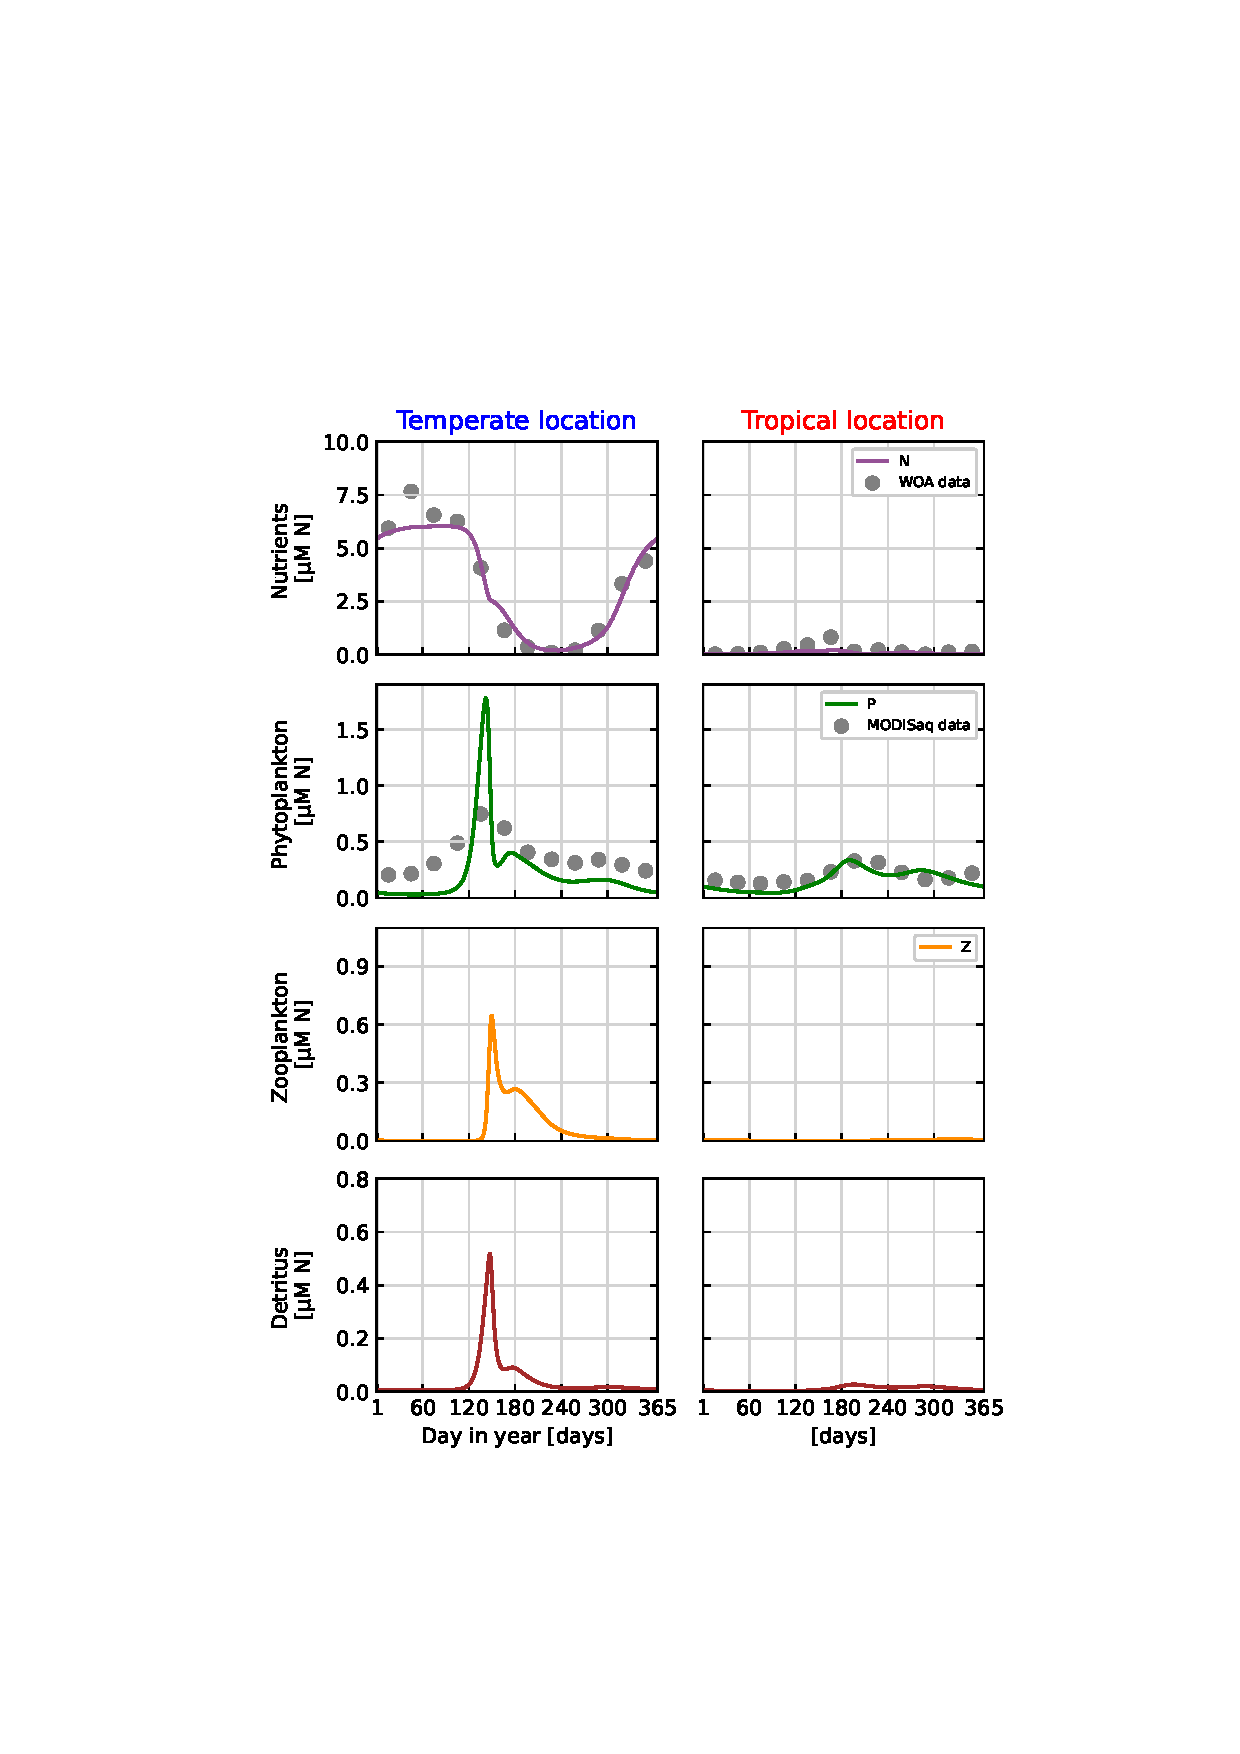
\includegraphics[width=6cm]{Figures/firstdraft_plots/02_NPZDslab.pdf}
\caption{Dynamics of NPZD slab model (i.e. use case 1) in the two exemplary locations. Output is the last year of a 5 year simulation with repeated climatological forcing. Forcing used is shown in Figure \ref{phydraforcing}. Grey dots are verification data from WOA 2018 and satellite climatology (see Section \ref{ForcingSection} for details).}
\label{Figure:NPZDslab_results}
\end{figure}

%%f
\begin{figure}[t]
\includegraphics[width=6cm]{Figures/firstdraft_plots/03_chemostat.pdf}
\caption{Phytoplankton and zooplankton biomass per size class under steady chemostat flow-through forcing. Panel (a) shows a detailed view of the first 2 years of simulation. Panel (b) shows 10 years of model time evolution of the same run as the model output approaches a steady state. Panel (c) shows zooplankton biomass time evolution for the same model run. Plot is a recreation (same model setup \& parameters) of a plot in \citet{Banas2011b}}
\label{Figure:chemostat_plot}
\end{figure}

%%f
\begin{figure*}[t]
\includegraphics[width=10cm]{Figures/firstdraft_schematics/03__schematics_SizeStructSlab.pdf}
\caption{Model schematic of size-structured \unit{NP_{20}Z_{20}} slab model for use case 3. The model is a combination of the size-structured food web of use case 2 and the detritus component and slab physical setting of use case 1. The model ecosystem is contained in the light-blue area, all open errors represent loss processes that are lost from the system.}
\label{Figure:phydraschematics_3}
\end{figure*}



%%f
\begin{figure*}[t]
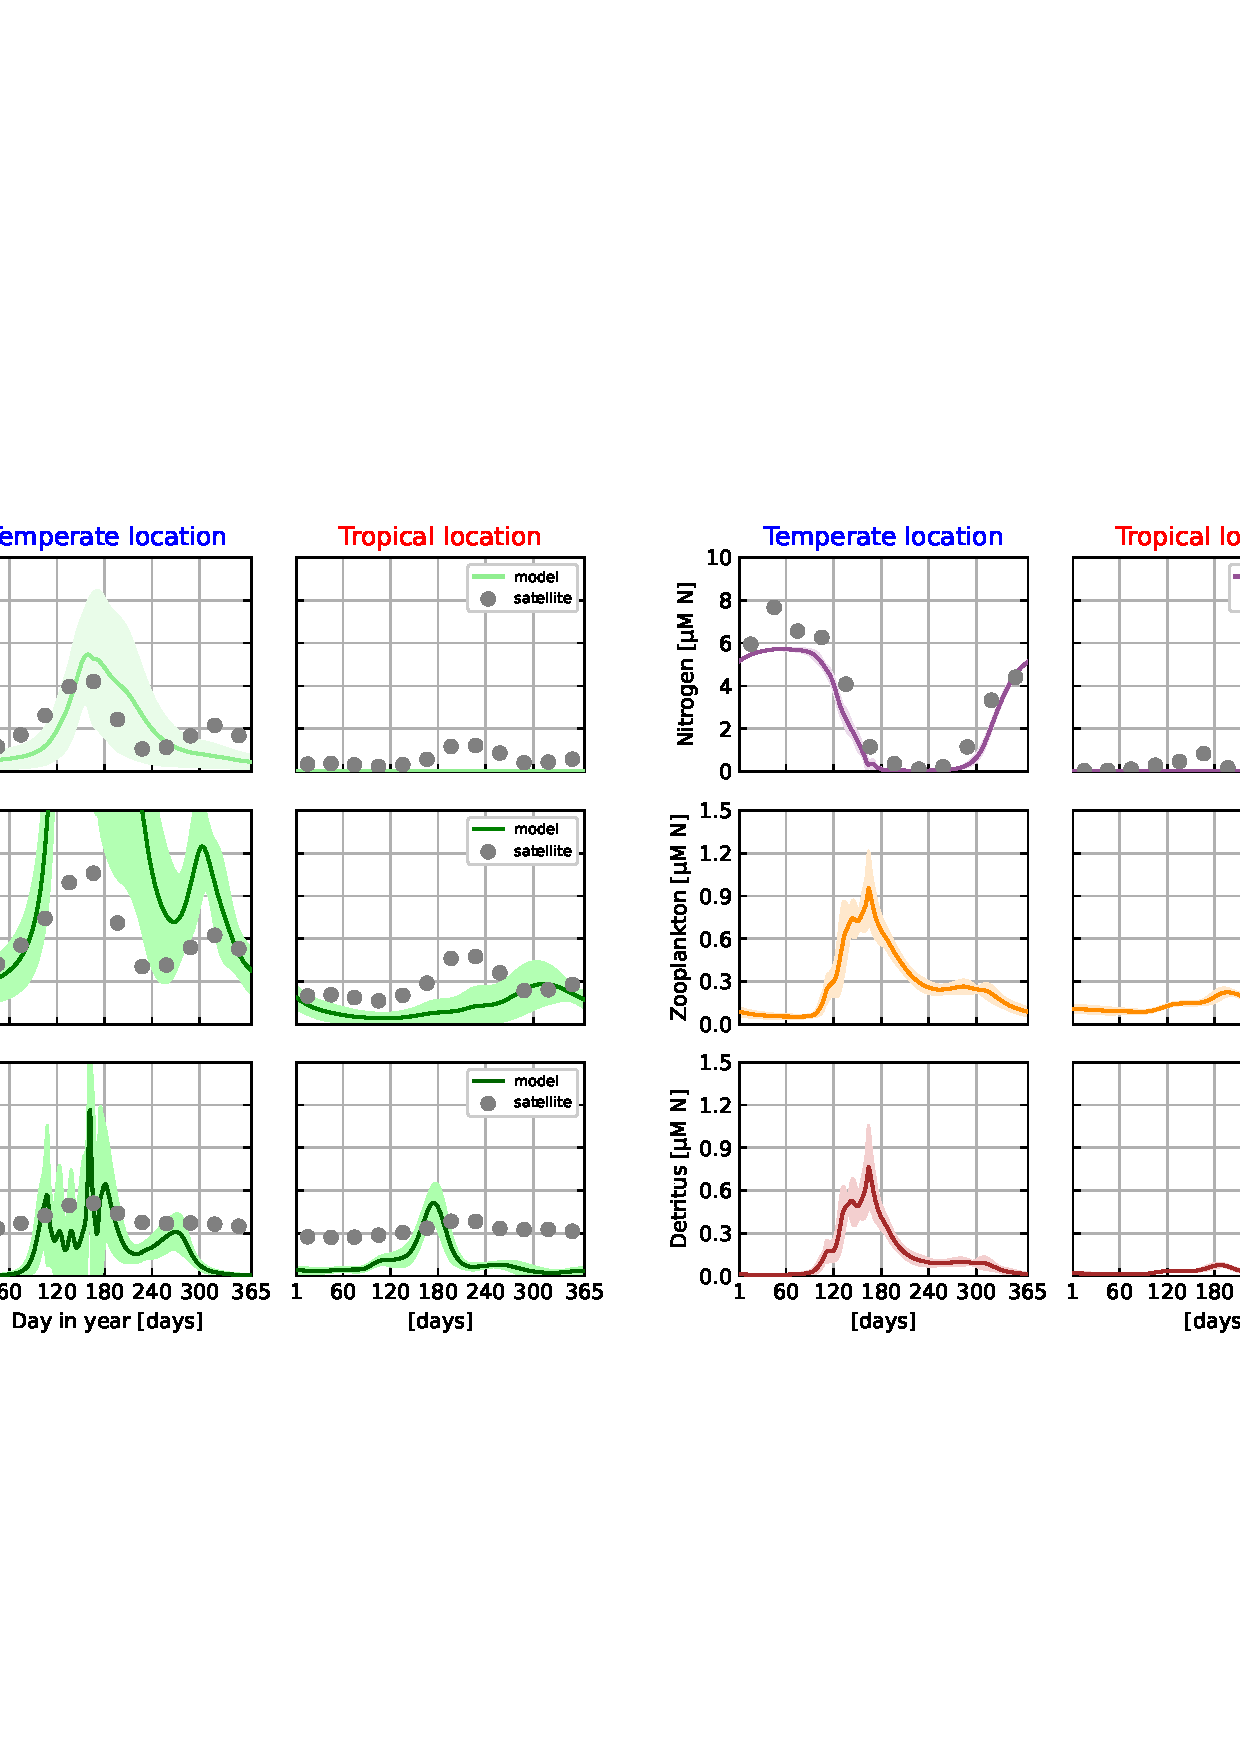
\includegraphics[width=12cm]{Figures/firstdraft_plots/04_sizestruct_slab.pdf}
\caption{Dynamics of size-structured \unit{NP_{20}Z_{20}D} slab model (i.e. use case 3) in the two exemplary locations. Solid line represents the mean dynamics of the last 10 years of a 20 year run with repeated climatological forcing, shaded areas show the standard deviation. Forcing used is shown in Figure \ref{phydraforcing}. Grey dots are verification data from WOA 2018 and satellite climatology (see Section \ref{ForcingSection} for details). Size ranges are picoplankton 0.5 - 2 \unit{\mu m}, nanoplankton 2 - 20 \unit{\mu m}, microplankton 20 - 50 \unit{\mu m}. Zooplankton dynamics shown are the sum of all size classes.}
\label{Figure:SizeStructuredSlab_results}
\end{figure*}
% Tables

\clearpage

% this is a custom function to be able to see references when rendering subfiles:
\biblio

\end{document}